% Shared section: why do Gallup and the WVS disagree? Wording vs. sampling
\subsection{Experimental effects of wording and scale}\label{subsec:experiment}

Table~\ref{tab:fabre_regressions} reports regressions of the answer on the randomized treatments, with country fixed effects, survey weights and heteroskedasticity-robust standard errors. The ladder wording shifts answers by \effectLadder points on average (s.e.\ \seLadder), i.e.\ respondents rate their lives lower on the ``best possible life'' ladder than when asked how satisfied they are. This is in line with evidence that the two questions elicit different considerations: in open-ended answers, the ladder evokes power and wealth more than life satisfaction does \citep{nilsson_cantril_2024}. The scale effect is smaller: answers on the 1--10 scale are \effectScale points higher than on the 0--10 scale (s.e.\ \seScale), which, once the 1--10 answers are linearly stretched to 0--10, amounts to \effectScaleZeroTen points. Wording and scale do not interact. Measured as the share of respondents answering 6 or more, the ladder changes the share ``satisfied'' by \effectLadderSatisfied percentage points.

\begin{table}[htbp]
    \centering
    \caption{Effects of question wording and scale on life evaluation, Fabre (2025) survey experiment}\label{tab:fabre_regressions}
    \begin{adjustbox}{max width=\textwidth}
    
\begingroup
\centering
\begin{tabular}{lcccccc}
   \tabularnewline \midrule \midrule
   Dependent Variables: & \multicolumn{2}{c}{Answer} & Answer (0--10 equiv.) & Satisfied (6+) & \multicolumn{2}{c}{Answer (0--10 equiv.)}\\
   Model:                                                                         & (1)            & (2)            & (3)            & (4)            & (5)            & (6)\\  
   \midrule
   \emph{Variables}\\
   Ladder wording (Gallup)                                                        & -0.451$^{***}$ & -0.455$^{***}$ & -0.456$^{***}$ & -0.088$^{***}$ & -0.464$^{***}$ & -0.494$^{**}$\\   
                                                                                  & (0.046)        & (0.067)        & (0.067)        & (0.013)        & (0.123)        & (0.172)\\   
   Scale 1--10                                                                    & 0.137$^{**}$   & 0.132          & -0.260$^{***}$ & -0.008         & -0.276$^{***}$ & -0.540$^{**}$\\   
                                                                                  & (0.046)        & (0.068)        & (0.072)        & (0.013)        & (0.046)        & (0.182)\\   
   Ladder wording (Gallup) $\times$ Scale 1--10                                   &                & 0.008          & -0.041         & 0.028          &                & 0.055\\   
                                                                                  &                & (0.092)        & (0.097)        & (0.019)        &                & (0.247)\\   
   Income quartile (1--4)                                                         &                &                &                &                & 0.689$^{***}$  & 0.635$^{***}$\\   
                                                                                  &                &                &                &                & (0.031)        & (0.043)\\   
   Income quartile (1--4) $\times$ Ladder wording (Gallup)                        &                &                &                &                & -0.004         & 0.009\\   
                                                                                  &                &                &                &                & (0.042)        & (0.058)\\   
   Income quartile (1--4) $\times$ Scale 1--10                                    &                &                &                &                &                & 0.106\\   
                                                                                  &                &                &                &                &                & (0.061)\\   
   Income quartile (1--4) $\times$ Ladder wording (Gallup) $\times$ Scale 1--10   &                &                &                &                &                & -0.022\\   
                                                                                  &                &                &                &                &                & (0.083)\\   
   \midrule
   \emph{Fixed-effects}\\
   Country                                                                        & Yes            & Yes            & Yes            & Yes            & Yes            & Yes\\  
   \midrule
   \emph{Fit statistics}\\
   Observations                                                                   & 11,000         & 11,000         & 11,000         & 11,000         & 11,000         & 11,000\\  
   R$^2$                                                                          & 0.05681        & 0.05681        & 0.05942        & 0.04208        & 0.15976        & 0.16024\\  
   \midrule \midrule
   \multicolumn{7}{l}{\emph{Heteroskedasticity-robust standard-errors in parentheses}}\\
   \multicolumn{7}{l}{\emph{Signif. Codes: ***: 0.001, **: 0.01, *: 0.05}}\\
\end{tabular}
\par\endgroup



    \end{adjustbox}
    \begin{minipage}{\textwidth}\footnotesize \textit{Note:} OLS with country fixed effects, survey weights (normalized within country) and heteroskedasticity-robust standard errors in parentheses. \textit{Ladder wording}: Cantril ladder (vs.\ WVS life satisfaction). \textit{Scale 1--10}: answers from 1 to 10 (vs.\ 0 to 10). In columns 3 and 5, 1--10 answers are linearly rescaled to 0--10. Column 5 interacts the wording with the respondent's income quartile within their country. * $p<.05$, ** $p<.01$, *** $p<.001$.\end{minipage}
\end{table}

Two further results matter for the interpretation of cross-country comparisons. First, the ladder does not steepen the income gradient \textit{within} countries: the interaction between ladder wording and the income quartile is \interactionLadderIncome ($p = \pInteractionLadderIncome$), against a gradient of \gradientIncomeSatisfaction points per quartile (column 5). So, at least among individuals in high-income countries, the ladder is not more ``about money'' than the satisfaction question. Second, the wording effect differs markedly across countries (Figure~\ref{fig:fabre_variants}). It ranges from \wordingMin points (Spain) to \wordingMax (Japan), where the ladder yields \textit{higher} answers than the satisfaction question, and the hypothesis of a common effect across countries is strongly rejected ($\chi^2(9) = \chiHeterogeneityWording$, $p < .001$). Question wording therefore affects not only the level but also the ranking of countries.

\begin{figure}[htbp]
    \centering
    \caption{Mean answer by question variant and country, Fabre (2025)}\label{fig:fabre_variants}
    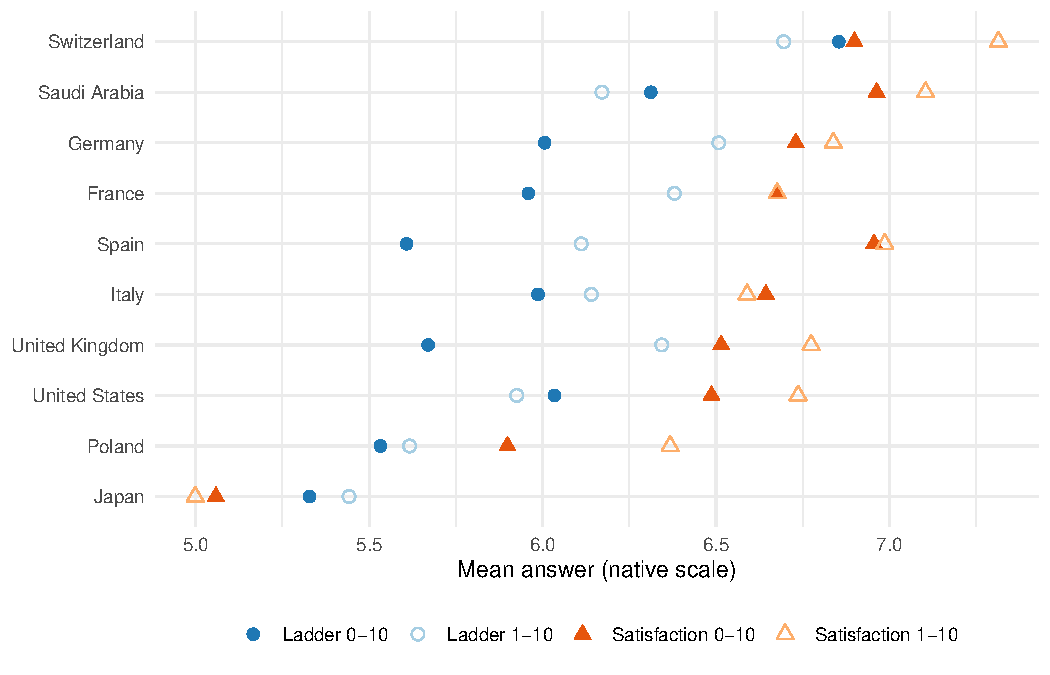
\includegraphics[width=.85\textwidth]{../figures/main/fabre_variants_by_country.pdf}
    \begin{minipage}{.85\textwidth}\footnotesize \textit{Note:} Weighted mean answer on the native scale of each variant (0--10 or 1--10).\end{minipage}
\end{figure}

\subsection{Decomposing the Gallup--WVS gap in ten countries}\label{subsec:decomposition}

For each country $c$ of the experiment, I define the observed gap between Gallup and the WVS as $D_c = G_c - W_c$, where $W_c$ is the mean satisfaction in the latest WVS survey of the country and $G_c$ the mean ladder in Gallup the same year (or the closest year, at most three years apart; seven countries have an exact match). Comparing the two datasets in the same year removes the influence of changes in well-being over time. The experiment measures, within the same sample, the \textit{question effect} $Q_c = F_c(\text{ladder 0--10}) - F_c(\text{satisfaction 1--10})$, where $F_c(v)$ is the mean answer to variant $v$ in country $c$. The residual $R_c = D_c - Q_c$ is the part of the gap due to everything that differs between the two datasets except the question: sampling frames, interview modes, questionnaire context, translations, and survey-specific time effects. This decomposition assumes that the question effect measured online in 2025 applies to the Gallup and WVS samples of earlier years.

Table~\ref{tab:decomposition_country} and Figure~\ref{fig:decomposition} present the decomposition for each country, and Table~\ref{tab:decomposition_summary} summarizes it with 95\% confidence intervals from a bootstrap that resamples respondents in the three surveys. On average, the gap between Gallup and WVS answers is $D = \decompMeanGap$ points. The question effect is even larger in absolute value: $Q = \decompMeanQuestion$ points. Wording (and scale) thus fully account for the fact that Gallup yields lower levels than the WVS in high-income countries, and the residual partly offsets it ($R = \decompMeanResidual$).

\begin{table}[htbp]
    \centering
    \caption{Decomposition of the Gallup--WVS gap by country}\label{tab:decomposition_country}
    \begin{adjustbox}{max width=\textwidth}
    \begin{tabular}{lllccccccc}
\toprule
Country & Year WVS/EVS (Gallup) & Survey: mode & Gallup & WVS/EVS & Gap $D$ & Ladder 0--10 & Satisf. 1--10 & Question effect $Q$ & Residual $R$ \\ & & & (1) & (2) & (1)$-$(2) & \multicolumn{2}{c}{Fabre (2025)} & & $D-Q$ \\
\midrule
Poland & 2017 & EVS: CAPI & 6.28 & 7.56 & \ensuremath{-}1.28 & 5.53 & 6.37 & \ensuremath{-}0.84 & \ensuremath{-}0.44 \\
Spain & 2017 & EVS: CAPI & 6.47 & 7.49 & \ensuremath{-}1.02 & 5.61 & 6.99 & \ensuremath{-}1.38 & 0.36 \\
Japan & 2019 & WVS: Mail & 5.94 & 6.76 & \ensuremath{-}0.82 & 5.33 & 5.00 & 0.33 & \ensuremath{-}1.15 \\
Italy & 2018 & EVS: CAPI & 6.69 & 7.28 & \ensuremath{-}0.59 & 5.99 & 6.59 & \ensuremath{-}0.60 & 0.01 \\
Germany & 2018 & WVS: CAPI & 7.15 & 7.74 & \ensuremath{-}0.58 & 6.01 & 6.84 & \ensuremath{-}0.83 & 0.25 \\
United Kingdom & 2022 & WVS: CAPI/Web/Mail & 6.76 & 7.32 & \ensuremath{-}0.56 & 5.67 & 6.77 & \ensuremath{-}1.10 & 0.55 \\
France & 2018 & EVS: CAPI & 6.79 & 7.26 & \ensuremath{-}0.47 & 5.96 & 6.68 & \ensuremath{-}0.72 & 0.25 \\
Switzerland & 2017 & EVS: Web/Mail/CAPI & 7.58 & 8.02 & \ensuremath{-}0.43 & 6.85 & 7.31 & \ensuremath{-}0.46 & 0.03 \\
Saudi Arabia & 2003 (2006) & WVS: Face-to-face & 7.06 & 7.28 & \ensuremath{-}0.23 & 6.31 & 7.10 & \ensuremath{-}0.79 & 0.57 \\
United States & 2017 & WVS: Web/Phone & 7.23 & 7.22 & 0.01 & 6.03 & 6.74 & \ensuremath{-}0.70 & 0.71 \\
\bottomrule
\end{tabular}

    \end{adjustbox}
    \begin{minipage}{\textwidth}\footnotesize \textit{Note:} Mean answers on native scales (Gallup: 0--10; WVS: 1--10). The Gallup year is given in parentheses when it differs from the WVS year. WVS mode: main interview mode(s) of the WVS survey (CAPI: computer-assisted personal interviews).\end{minipage}
\end{table}

\begin{figure}[htbp]
    \centering
    \caption{Observed Gallup--WVS gap, question effect and residual by country}\label{fig:decomposition}
    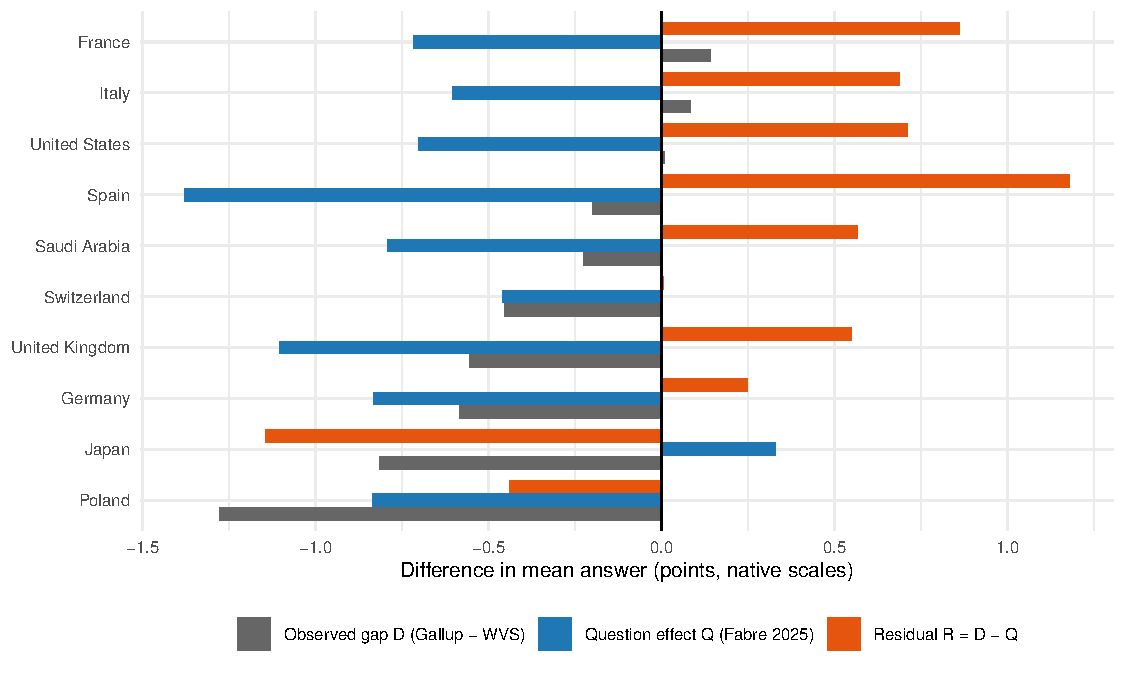
\includegraphics[width=.9\textwidth]{../figures/main/decomposition_by_country.pdf}
\end{figure}

What matters for correlations with GDP and for country rankings, however, is not the average gap but its variation across countries. Here, the question effect explains nothing: the covariance between $D_c$ and $Q_c$ is slightly negative, so that the share of the cross-country variance of the gap attributable to the question, $\mathrm{cov}(D,Q)/\mathrm{var}(D)$, is \decompVarShareQuestion (95\% CI [\decompLowVarShareQuestion; \decompHighVarShareQuestion]), and the residual accounts for the rest. Predicting a country's Gallup score by adding its experimentally measured question effect to its WVS score does worse (root mean squared error: \decompRmsePredictionGallup) than simply adding the average gap (\decompRmseNaive). The conclusion is the same when restricting to the \nSameYear countries where Gallup and WVS are observed the same year (variance share: \varShareQuestionSameYear) or to the \nRecent countries with a WVS survey since 2017 (\varShareQuestionRecent), and for the share of respondents answering 6 or more (\decompVarShareQuestionSat). For instance, the question effect is largest in Spain and the United Kingdom, but the observed gap is small in Spain; Japan is the only country with a positive question effect, but the gap is negative there.

\begin{table}[htbp]
    \centering
    \caption{Decomposition of the Gallup--WVS gap: summary}\label{tab:decomposition_summary}
    \begin{adjustbox}{max width=\textwidth}
    \begin{tabular}{lc}
\toprule
Statistic & Estimate [95\% bootstrap CI] \\
\midrule
Mean gap $D$ (Gallup $-$ WVS) & \ensuremath{-}0.60 [\ensuremath{-}0.64; \ensuremath{-}0.55] \\
Mean question effect $Q$ (wording + scale) & \ensuremath{-}0.71 [\ensuremath{-}0.84; \ensuremath{-}0.56] \\
Mean residual $R$ (sampling, mode, context) & 0.11 [\ensuremath{-}0.04; 0.26] \\
\midrule
Share of mean gap due to question ($\bar Q/\bar D$) & 1.19 [0.94; 1.45] \\
Share of gross level difference due to question ($|\bar Q|/(|\bar Q|+|\bar R|)$) & 0.86 [0.76; 0.99] \\
Same, country average ($\overline{|Q_c|/(|Q_c|+|R_c|)}$) & 0.69 [0.56; 0.72] \\
\midrule
Share of cross-country variance of $D$ due to $Q$ ($\mathrm{cov}(D,Q)/\mathrm{var}(D)$) & 0.11 [\ensuremath{-}0.33; 0.55] \\
Share of cross-country variance of $D$ due to $R$ & 0.89 [0.45; 1.33] \\
Mean absolute gap $|D|$ & 0.60 [0.56; 0.65] \\
Mean absolute residual $|R|$ & 0.43 [0.33; 0.60] \\
Correlation between $D$ and $Q$ & 0.09 [\ensuremath{-}0.26; 0.41] \\
\midrule
Mean gap, share satisfied (6+) & \ensuremath{-}0.07 [\ensuremath{-}0.08; \ensuremath{-}0.06] \\
Mean question effect, share satisfied (6+) & \ensuremath{-}0.11 [\ensuremath{-}0.14; \ensuremath{-}0.08] \\
Variance share due to $Q$, share satisfied & 0.04 [\ensuremath{-}0.33; 0.45] \\
\bottomrule
\end{tabular}

    \end{adjustbox}
    \begin{minipage}{\textwidth}\footnotesize \textit{Note:} \nDecompCountries countries. 95\% confidence intervals from 1,000 bootstrap replications resampling respondents within country $\times$ variant (Fabre), within country (WVS), and answers within country (Gallup, multinomial).\end{minipage}
\end{table}

Two direct comparisons of samples asked the same question corroborate the importance of the residual. First, Gallup respondents (World Happiness Report, 2023--2025) rate their lives \meanSampleEffectGallup points higher on the 0--10 ladder than Fabre (2025) online respondents asked the same question, with differences ranging from \minSampleEffectGallup to \maxSampleEffectGallup across countries. Second, WVS respondents report \meanSampleEffectWVS points higher satisfaction than online respondents asked the WVS question (this comparison also includes changes over time, as WVS surveys are older). These sample (and mode) effects are of the same order of magnitude as the question effect, and they vary across countries. Even in the United States, where the 2017 WVS was itself conducted online, WVS respondents report \sampleEffectUSWVS points higher satisfaction than Fabre (2025) respondents.

\subsection{The global discrepancy}\label{subsec:global_gap}

The ten countries of the experiment are all high-income, whereas the Gallup--WVS discrepancy matters most for the global relation between GDP and well-being. Restricting both datasets to the \nCommon country-years (\nCommonCountries countries) observed by both surveys the same year, log GDP explains \RtwoCommonGallup of the variance of Gallup's mean ladder but only \RtwoCommonWVS of WVS mean satisfaction, and income accounts for \shareIncomeCommonGallup\% of the variance explained jointly with region in Gallup against \shareIncomeCommonWVS\% in the WVS. The gap between the two datasets increases strongly with GDP (Figure~\ref{fig:gap_gdp}): the slope is \slopeGapGDP per unit of $\log_{10}$ GDP (s.e.\ \seSlopeGapGDP, clustered by country), with WVS answers exceeding Gallup answers by around two points in low-income countries, against less than half a point in high-income countries.

\begin{figure}[htbp]
    \centering
    \caption{Gallup ladder minus WVS satisfaction in the same country-year, by GDP per capita}\label{fig:gap_gdp}
    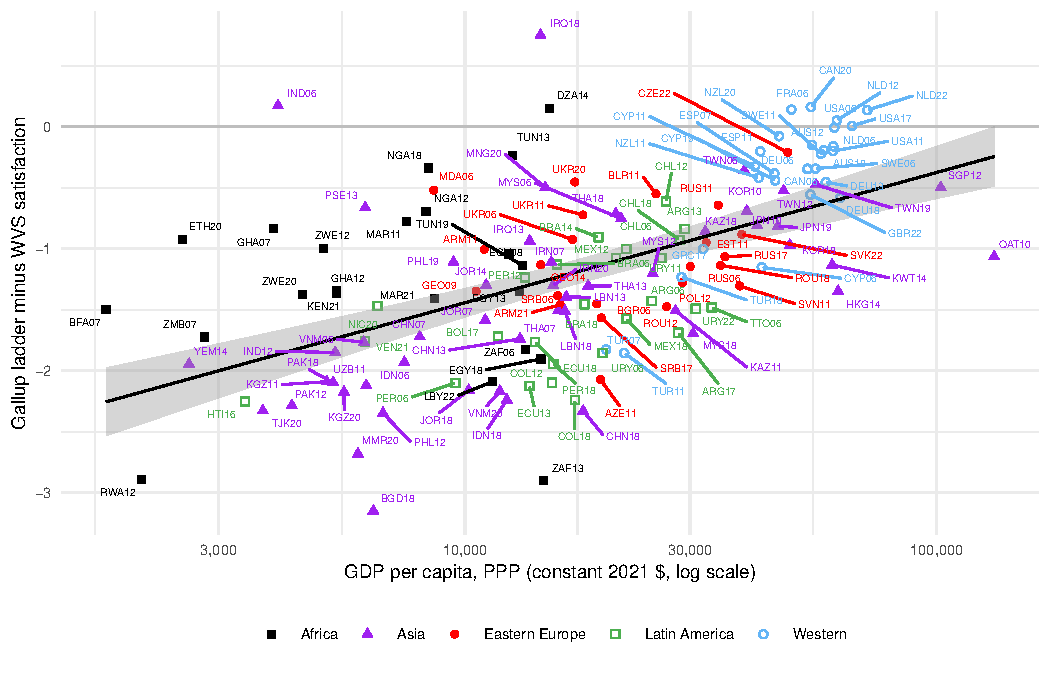
\includegraphics[width=.9\textwidth]{../figures/main/gap_gallup_wvs_vs_gdp.pdf}
    \begin{minipage}{.9\textwidth}\footnotesize \textit{Note:} Mean answers on native scales (Gallup: 0--10; WVS: 1--10), \nCommon country-years observed by both surveys. Line: OLS fit with 95\% confidence band.\end{minipage}
\end{figure}

Could the question explain this pattern? Within the experiment, the question effect is not significantly related to GDP (slope \slopeQuestionGDP, s.e.\ \seSlopeQuestionGDP), which is unsurprising given the narrow range of GDP among the ten countries. Even taking this point estimate at face value and extrapolating it to all countries, adjusting WVS answers for the predicted question effect would raise the $R^2$ of WVS satisfaction on log GDP only from \RtwoCommonWVS to \RtwoAdjustedWVS, far from Gallup's \RtwoCommonGallup. The experiment cannot rule out that the wording effect is much larger in low-income countries---for instance if the ``best possible life'' evokes material comparisons more strongly where material deprivation is widespread---but nothing in the high-income evidence points in that direction: the ladder does not steepen the individual income gradient (Section~\ref{subsec:experiment}), and the country-level question effects are unrelated to the observed gaps.
